\section{Hiện thực hệ thống}
\subsection{Hiện thực phần cứng}

Hệ thống được hiện thực phần cứng thông qua sự tích hợp của nhiều thành phần điện tử, đảm bảo khả năng thu thập, xử lý tín hiệu và truyền dữ liệu một cách hiệu quả. Mục tiêu chính của phần cứng là cung cấp nền tảng ổn định, chính xác cho việc nhận diện cử chỉ ngôn ngữ ký hiệu.

\subsubsection{Các thành phần phần cứng chính}

\begin{itemize}
    \item \textbf{Cảm biến Flex:}
    \begin{itemize}
        \item \textit{Chức năng:} Đo độ uốn cong của các ngón tay, phản ánh cử chỉ của bàn tay. Khi uốn cong, giá trị điện trở của cảm biến thay đổi, từ đó tạo ra tín hiệu điện áp tương ứng.
        \item \textit{Đặc điểm:}
        \begin{itemize}
            \item Giá trị điện trở thay đổi từ 25k$\Omega$ (khi thẳng) đến hơn 100k$\Omega$ (khi uốn cong 90°).
            \item Được kết nối với vi điều khiển qua mạch chia điện áp để chuyển đổi tín hiệu thành dữ liệu số.
        \end{itemize}
    \end{itemize}

    \item \textbf{Vi điều khiển Arduino LilyPad:}
    \begin{itemize}
        \item \textit{Chức năng:} Là trung tâm xử lý tín hiệu từ cảm biến Flex, cảm biến con quay hồi chuyển và điều khiển các thành phần khác.
        \item \textit{Đặc điểm kỹ thuật:}
        \begin{itemize}
            \item Sử dụng vi điều khiển ATmega328 với 14 chân I/O số, 6 chân đầu vào analog.
            \item Kích thước nhỏ gọn, phù hợp với các thiết bị đeo.
        \end{itemize}
    \end{itemize}

    \item \textbf{Mô-đun Bluetooth HC-05:}
    \begin{itemize}
        \item \textit{Chức năng:} Truyền dữ liệu không dây từ hệ thống đến các thiết bị đầu cuối như điện thoại hoặc máy tính để xử lý và hiển thị.
        \item \textit{Đặc điểm:}
        \begin{itemize}
            \item Hỗ trợ giao tiếp trong phạm vi 10m.
            \item Giao tiếp với Arduino thông qua các chân TX và RX.
        \end{itemize}
    \end{itemize}

    \item \textbf{Cảm biến con quay hồi chuyển ITG-3200:}
    \begin{itemize}
        \item \textit{Chức năng:} Đo gia tốc và góc quay của bàn tay, hỗ trợ nhận diện cử chỉ một cách chính xác hơn.
        \item \textit{Đặc điểm:}
        \begin{itemize}
            \item Giao tiếp qua giao thức I2C.
            \item Được sử dụng để bổ sung thông tin về chuyển động của bàn tay.
        \end{itemize}
    \end{itemize}

    \item \textbf{Mô-đun TCA9548A:}
    \begin{itemize}
        \item \textit{Chức năng:} Là bộ chuyển mạch I2C 8 kênh, cho phép kết nối nhiều thiết bị I2C với cùng địa chỉ, tránh xung đột khi sử dụng nhiều cảm biến.
        \item \textit{Đặc điểm:}
        \begin{itemize}
            \item Hỗ trợ tối đa 8 thiết bị trên một bus I2C.
            \item Hoạt động ở điện áp từ 1.8V đến 5V.
        \end{itemize}
    \end{itemize}

    \item \textbf{Nguồn pin LiPo (Lithium Polymer):}
    \begin{itemize}
        \item \textit{Chức năng:} Cung cấp năng lượng cho toàn bộ hệ thống.
        \item \textit{Đặc điểm:}
        \begin{itemize}
            \item Điện áp đầu ra danh định 3.7V.
            \item Nhỏ gọn, dễ dàng tích hợp vào các thiết bị di động.
        \end{itemize}
    \end{itemize}

    \item \textbf{LED và điện trở:}
    \begin{itemize}
        \item LED: Hiển thị trạng thái hoạt động của hệ thống.
        \item Điện trở: Được sử dụng để điều chỉnh tín hiệu từ cảm biến Flex và giới hạn dòng qua LED.
    \end{itemize}
\end{itemize}

\subsubsection{Sơ đồ kết nối mạch}

\begin{figure}[H]
    \centering
    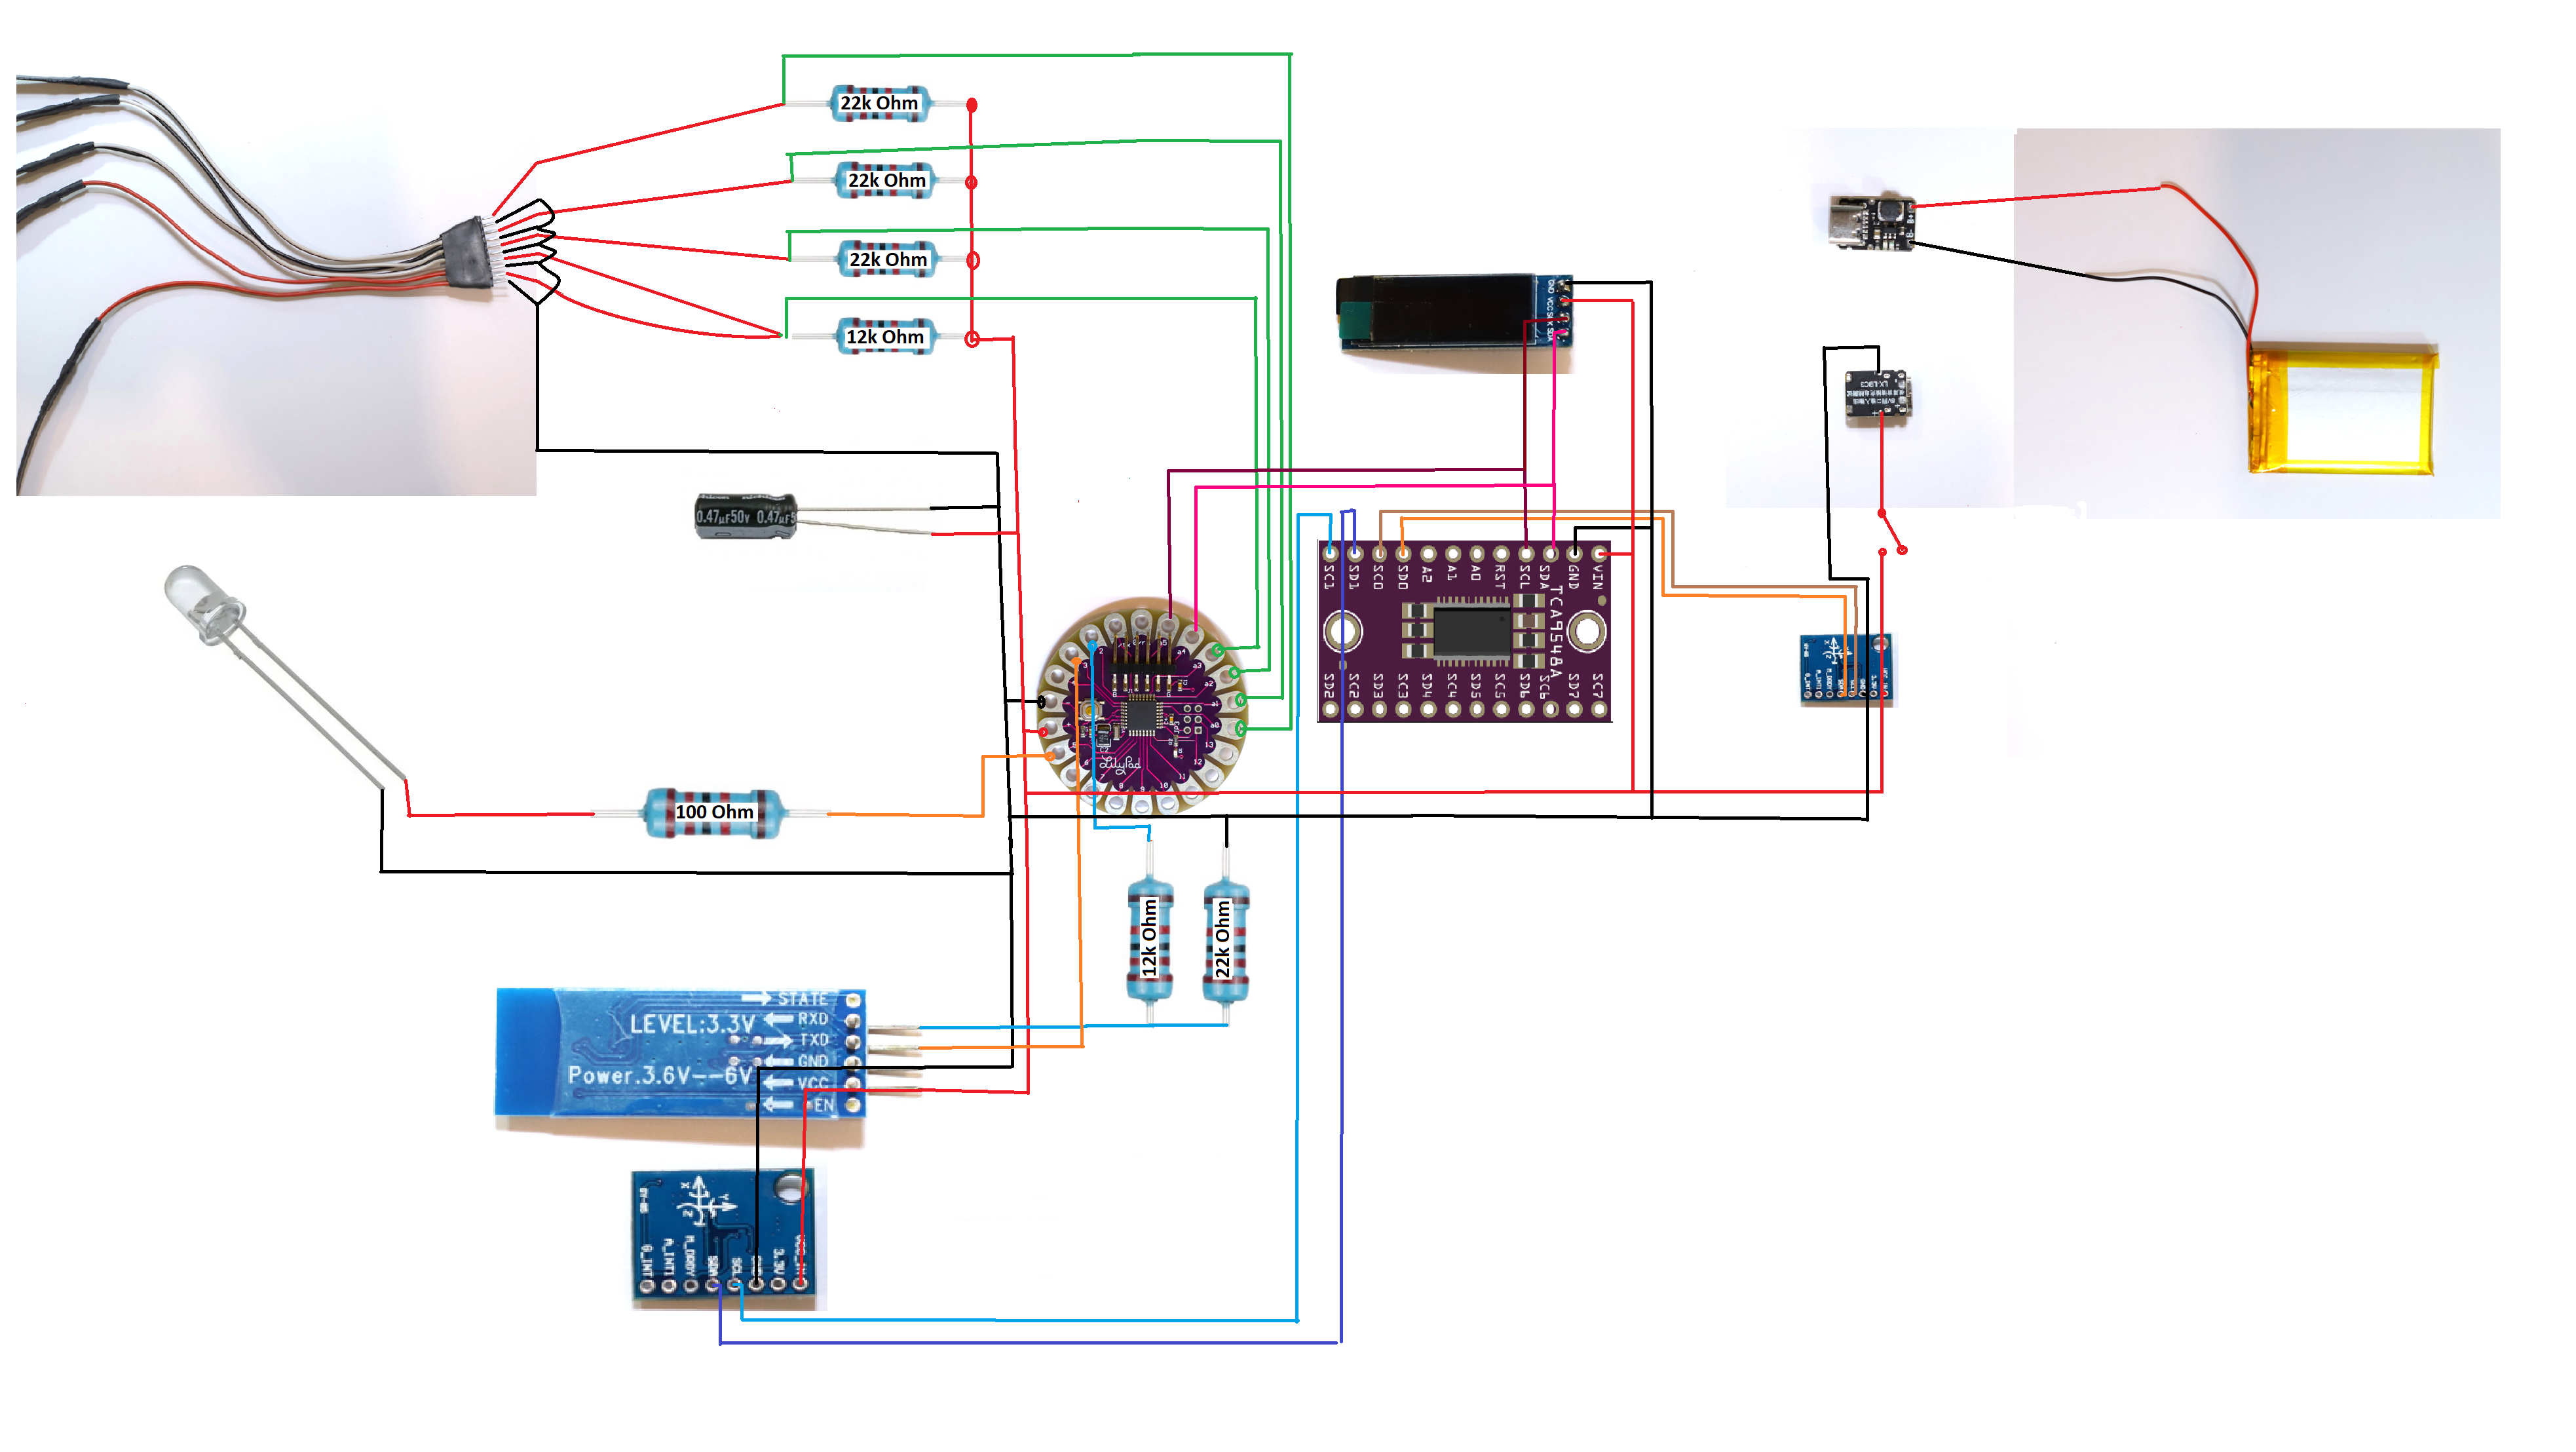
\includegraphics[width=\textwidth,height=\textheight,keepaspectratio]{Images/SystemImpl/schematic.png}
    \caption{Sơ đồ kết nối mạch}
    \label{fig:enter-label}
\end{figure}

\begin{itemize}
    \item \textbf{Kết nối cảm biến Flex với Arduino LilyPad:}
    \begin{itemize}
        \item Các cảm biến Flex được nối với chân analog của Arduino thông qua mạch chia điện áp (điện trở 22kΩ và 12kΩ).
        \item Tín hiệu điện trở từ cảm biến được chuyển thành điện áp và đưa vào Arduino để xử lý.
    \end{itemize}

    \item \textbf{Kết nối mô-đun Bluetooth HC-05 với Arduino LilyPad:}
    \begin{itemize}
        \item Chân TX của HC-05 nối với RX của Arduino và ngược lại (RX của HC-05 nối với TX của Arduino).
        \item Chân VCC và GND của HC-05 được nối với nguồn từ Arduino.
    \end{itemize}

    \item \textbf{Kết nối cảm biến ITG-3200 với TCA9548A:}
    \begin{itemize}
        \item Cảm biến ITG-3200 được nối vào các kênh riêng biệt của TCA9548A qua giao thức I2C.
        \item SDA và SCL của cảm biến được kết nối với các chân tương ứng trên TCA9548A.
    \end{itemize}

    \item \textbf{Kết nối TCA9548A với Arduino LilyPad:}
    \begin{itemize}
        \item Chân SDA và SCL của TCA9548A được nối với SDA và SCL trên Arduino.
        \item Chân VCC và GND của TCA9548A được nối với nguồn từ Arduino.
    \end{itemize}

    \item \textbf{Kết nối nguồn pin LiPo và LED:}
    \begin{itemize}
        \item Pin LiPo kết nối với cổng nguồn trên Arduino.
        \item LED được nối qua điện trở với chân I/O của Arduino để hiển thị trạng thái hoạt động.
    \end{itemize}
\end{itemize}

\subsubsection{Nhiệm vụ của phần cứng}

\begin{itemize}
    \item \textbf{Thu thập dữ liệu:}
    \begin{itemize}
        \item Cảm biến Flex cung cấp thông tin về độ uốn cong của ngón tay.
        \item Cảm biến ITG-3200 bổ sung dữ liệu về chuyển động và góc quay của bàn tay.
    \end{itemize}

    \item \textbf{Xử lý và truyền dữ liệu:}
    \begin{itemize}
        \item Arduino LilyPad xử lý dữ liệu từ các cảm biến và truyền đến các thiết bị đầu cuối qua Bluetooth HC-05.
    \end{itemize}

    \item \textbf{Quản lý giao tiếp I2C:}
    \begin{itemize}
        \item TCA9548A giải quyết vấn đề xung đột địa chỉ I2C khi sử dụng nhiều cảm biến.
    \end{itemize}

    \item \textbf{Hiển thị trạng thái:}
    \begin{itemize}
        \item LED hiển thị trạng thái hoạt động, màn hình OLED cung cấp thông tin trực quan.
    \end{itemize}
\end{itemize}

\subsubsection{Tóm tắt}

Hệ thống phần cứng được thiết kế để thu thập, xử lý và truyền dữ liệu phục vụ nhận diện cử chỉ ngôn ngữ ký hiệu. Các cảm biến Flex và ITG-3200 cung cấp thông tin về độ uốn cong và chuyển động bàn tay, trong khi Arduino LilyPad đóng vai trò trung tâm xử lý và điều khiển các thành phần khác. Mô-đun TCA9548A hỗ trợ quản lý giao tiếp I2C hiệu quả, và Bluetooth HC-05 đảm bảo truyền dữ liệu không dây. Toàn bộ hệ thống được tối ưu hóa về hiệu suất, đảm bảo hoạt động chính xác và ổn định trong thực tế.


\begin{figure}[H]
    \centering
    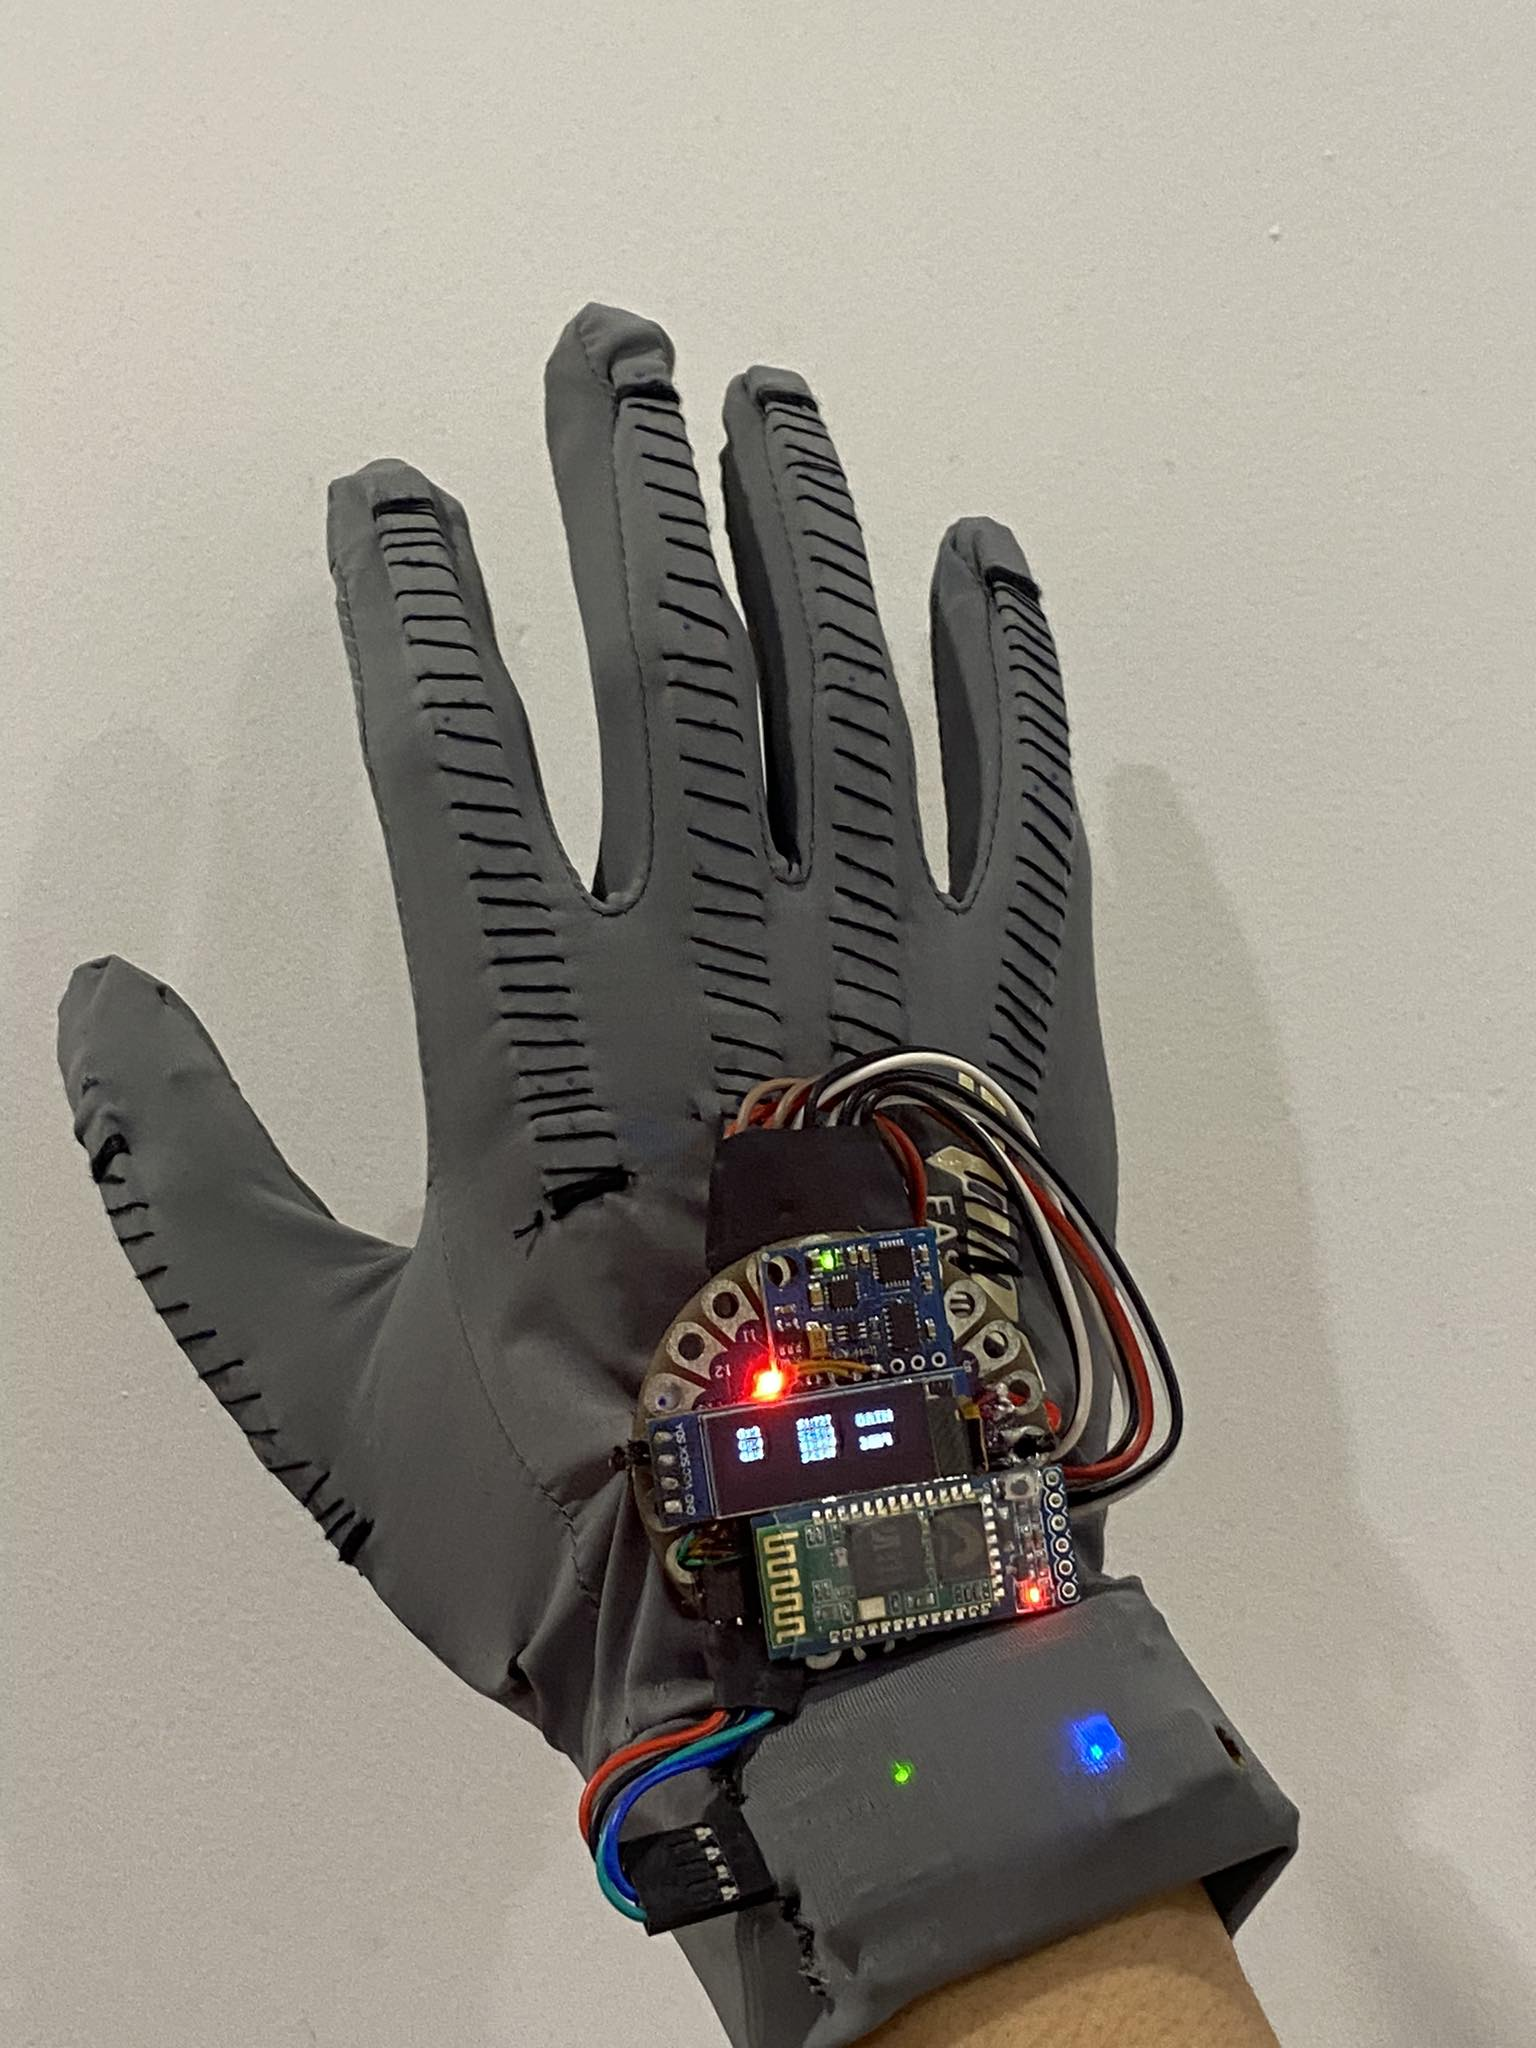
\includegraphics[width=\textwidth,height=\textheight,keepaspectratio]{Images/SystemImpl/full.jpg}
    \caption{Hình ảnh phần cứng sau khi hoàn thiện}
    \label{fig:enter-label}
\end{figure}

\subsection{Xây dựng bộ dữ liệu}

Phần xây dựng bộ dữ liệu tập trung vào thu thập và xử lý tín hiệu từ phần cứng nhằm tạo ra tập dữ liệu phục vụ huấn luyện và kiểm tra mô hình nhận diện cử chỉ ngôn ngữ ký hiệu.

\subsubsection{Thu thập dữ liệu từ phần cứng}

Dữ liệu được thu thập từ các cảm biến gia tốc và cảm biến Flex, kết nối với vi điều khiển Arduino LilyPad và truyền qua mô-đun Bluetooth HC-05 đến máy tính.

\begin{itemize}
    \item \textbf{Cấu trúc tín hiệu đầu vào:}
    \begin{itemize}
        \item Gia tốc trên các trục X, Y, Z: Cung cấp thông tin về chuyển động của bàn tay.
        \item Tín hiệu analog từ cảm biến Flex 1, 2, 3, 4: Đo độ uốn cong của các ngón tay.
        \item Cách kết nối:
        \begin{itemize}
            \item Flex 1 và Flex 2 (ngón trỏ và ngón cái) được nối song song, sau đó nối với chân A0 của Arduino.
            \item Các Flex còn lại được nối tuần tự vào các chân analog khác (A1, A2, A3).
        \end{itemize}
    \end{itemize}

    \item \textbf{Định dạng dữ liệu truyền:}
    \begin{itemize}
        \item Dữ liệu được gửi qua Bluetooth với định dạng chuỗi:
        \begin{figure}[H]
            \centering
            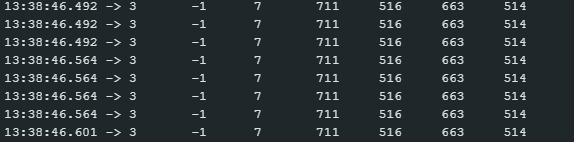
\includegraphics[width=\textwidth,height=\textheight,keepaspectratio]{Images/SystemImpl/data.png}
            \caption{Dạng dữ liêu được gửi}
            \label{fig:enter-label}
        \end{figure}
        \item Trong đó:
        \begin{itemize}
            \item Ba giá trị đầu là gia tốc trên các trục X, Y, Z.
            \item Bốn giá trị tiếp theo là tín hiệu analog từ các cảm biến Flex.
        \end{itemize}
        \item Tần suất gửi dữ liệu là mỗi 10ms một lần.
    \end{itemize}

    \item \textbf{Thu thập dữ liệu qua chương trình Python:}
    \begin{itemize}
        \item Chương trình Python giao tiếp với mô-đun Bluetooth HC-05 qua cổng COM.
        \item Tín hiệu nhận được từ Bluetooth được đọc, phân tách và lưu trữ dưới dạng có cấu trúc.
    \end{itemize}
\end{itemize}

\subsubsection{Xử lý và lưu trữ dữ liệu}

\begin{itemize}
    \item \textbf{Xử lý dữ liệu:}
    \begin{itemize}
        \item Các giá trị nhận được từ phần cứng được kiểm tra định dạng và chuyển đổi sang kiểu số nguyên.
        \item Mỗi hàng có 240*7 cột dữ liệu.
    \end{itemize}

    \item \textbf{Lưu trữ dữ liệu:}
    \begin{itemize}
        \item \textbf{Dữ liệu huấn luyện và kiểm tra:}
        \begin{itemize}
            \item Các chuỗi dữ liệu được lưu vào các tệp riêng biệt:
            \begin{itemize}
                \item \texttt{trainx}: Dữ liệu đầu vào cho huấn luyện.
                \item \texttt{testx}: Dữ liệu đầu vào cho kiểm tra.
            \end{itemize}
            \item Nhãn tương ứng (\texttt{trainy}, \texttt{testy}) được lưu kèm theo.
        \end{itemize}
        \item Dữ liệu được tổ chức dưới dạng từng dòng, mỗi dòng là một chuỗi giá trị đầy đủ.
    \end{itemize}

    \item \textbf{Thông số mỗi lần thu thập:}
    \begin{itemize}
        \item Số mẫu huấn luyện: 200.
        \item Số mẫu kiểm tra: 50.
        \item Tổng thời gian thu thập dữ liệu được xác định bởi số mẫu và tần suất gửi tín hiệu.
    \end{itemize}
\end{itemize}

\subsubsection{Tóm tắt}

Quy trình xây dựng bộ dữ liệu đảm bảo thu thập đầy đủ và chính xác tín hiệu từ phần cứng, với cấu trúc rõ ràng và dễ sử dụng. Bộ dữ liệu này là cơ sở quan trọng để huấn luyện mô hình học máy, hỗ trợ nhận diện chính xác các cử chỉ ngôn ngữ ký hiệu.

\begin{longtblr}[
    caption = {Định nghĩa các hành động},
  ]{
    width = \linewidth,
    colspec = {Q[404]Q[521]},
    hlines,
    vlines,
  }
  Label 0 & Xin chào\\
  Label 1& Tôi\\
  Label 2&Tên\\
  Label 3&Tiến\\
  Label 4&Tạm biệt\\
\end{longtblr}

\begin{figure}[H]
    \centering
    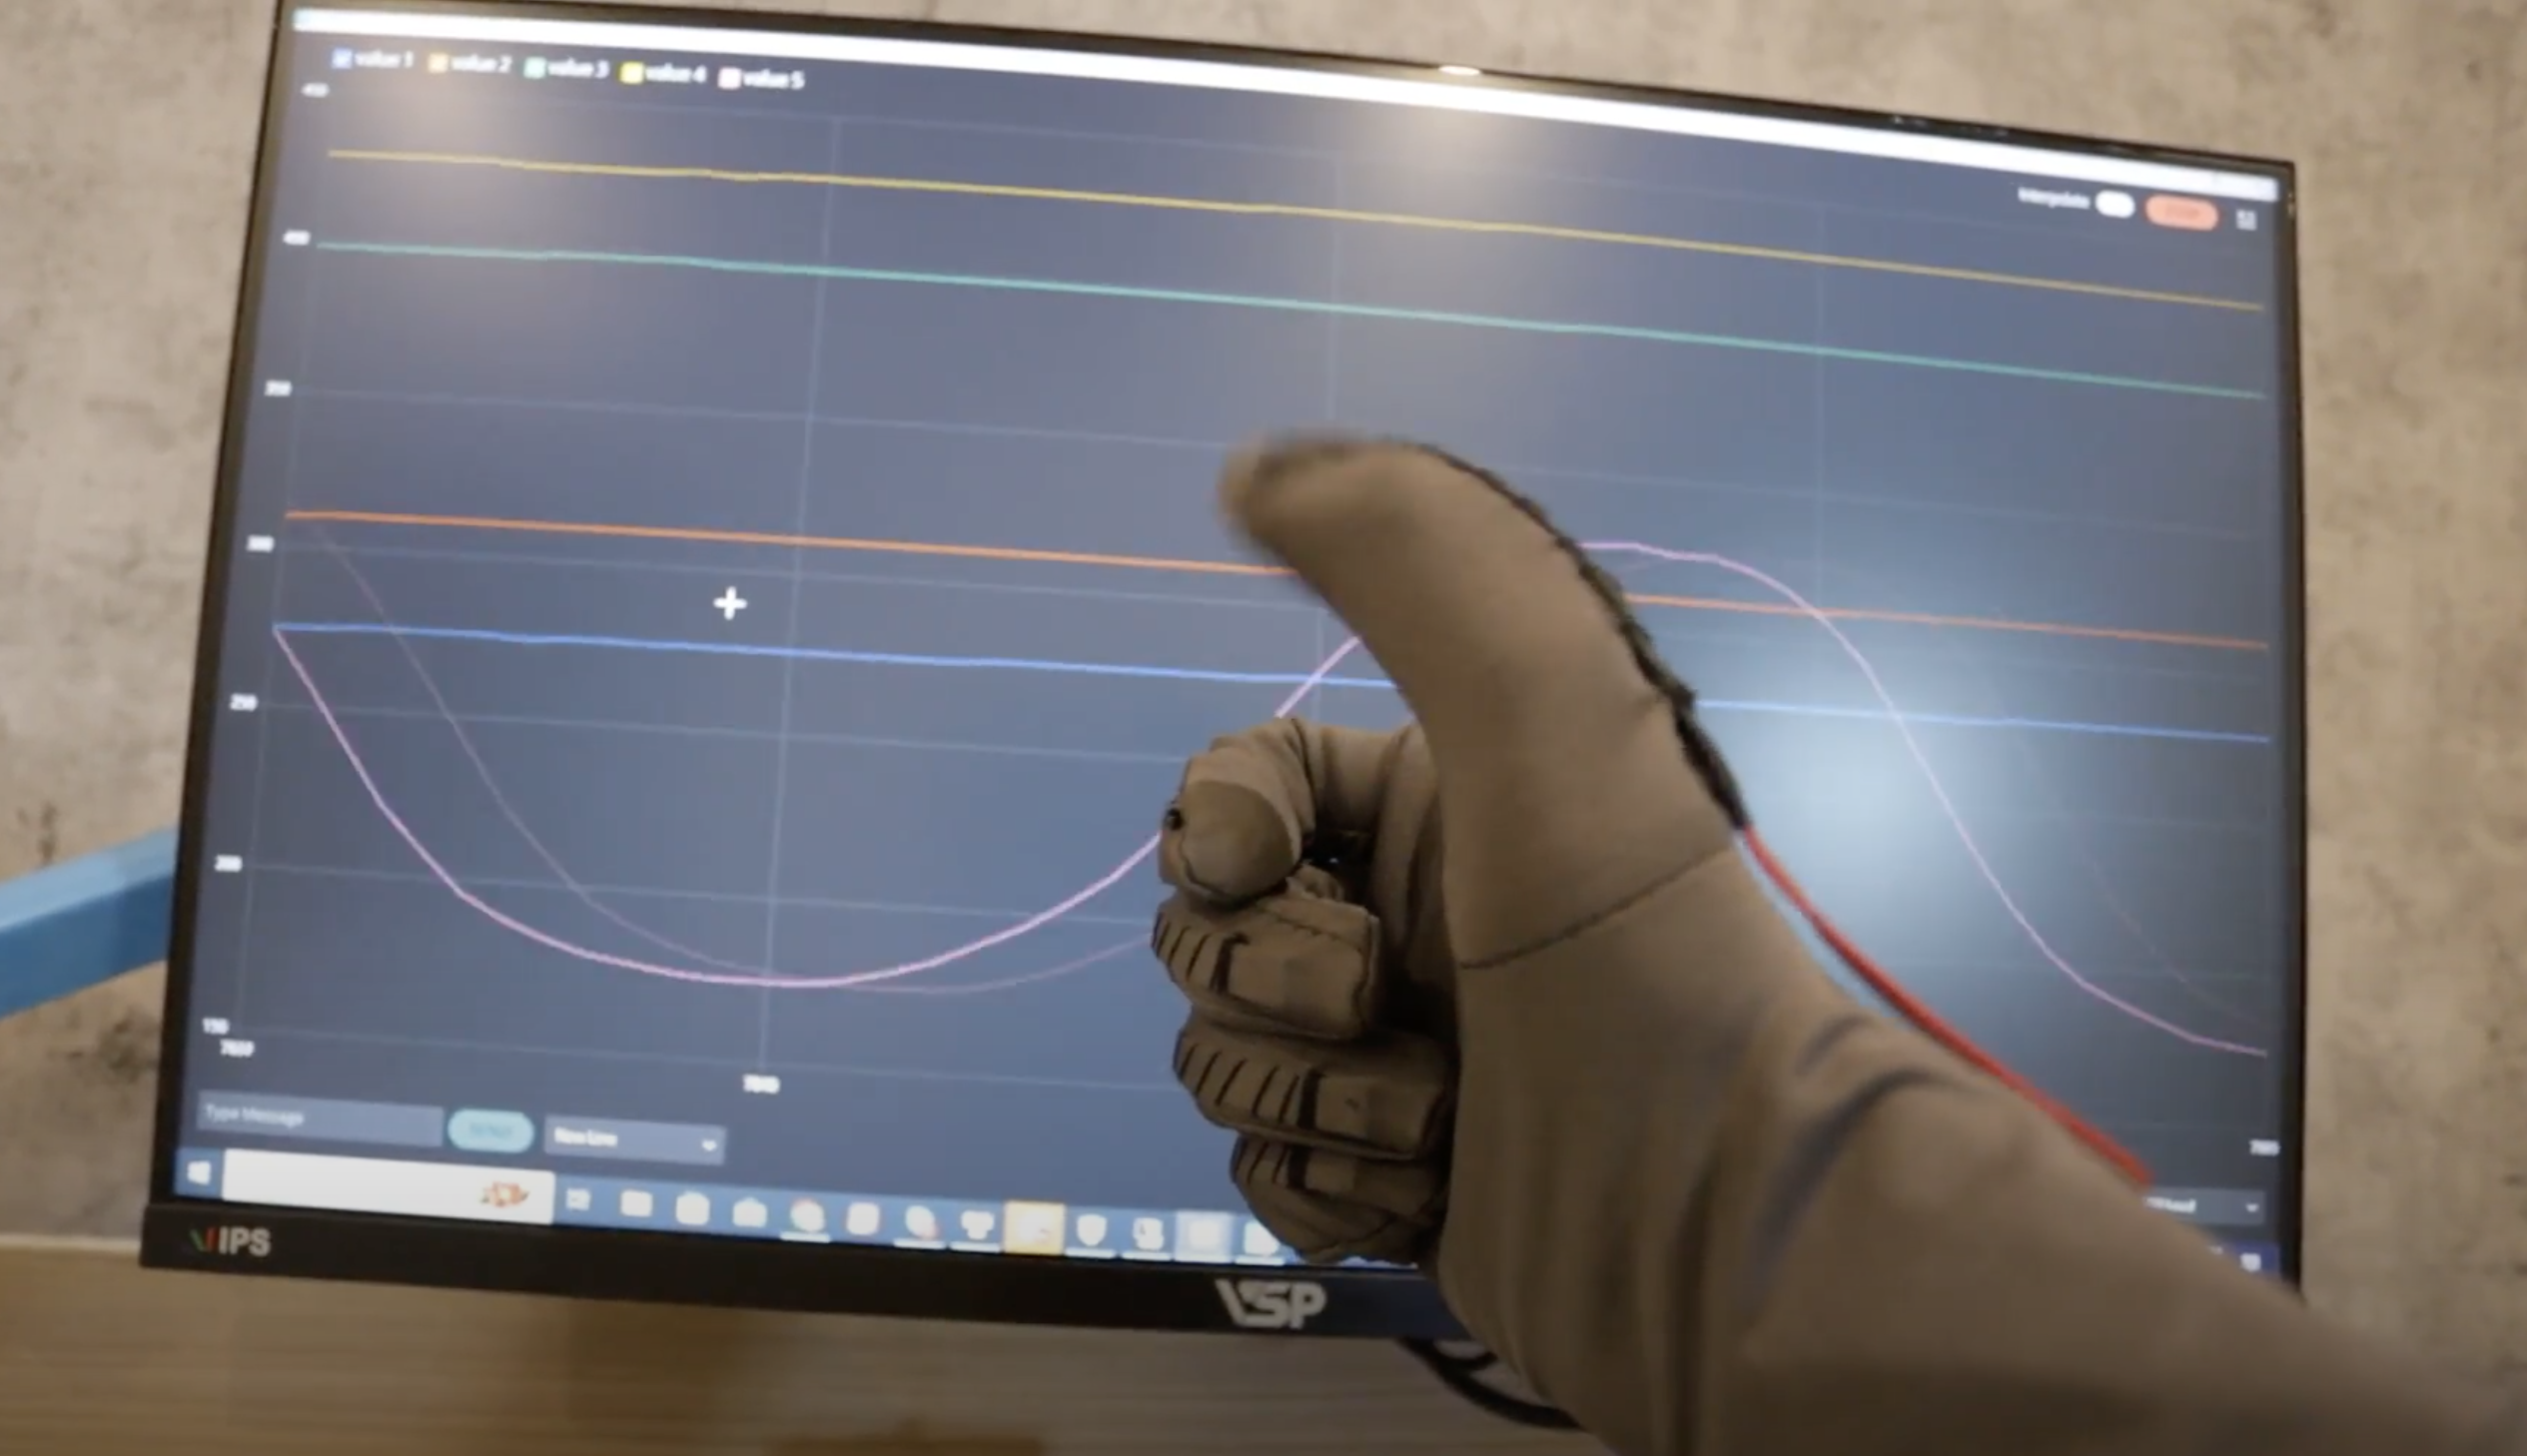
\includegraphics[width=10cm]{Images/SystemImpl/readdt_result_1.png}
    \centering
    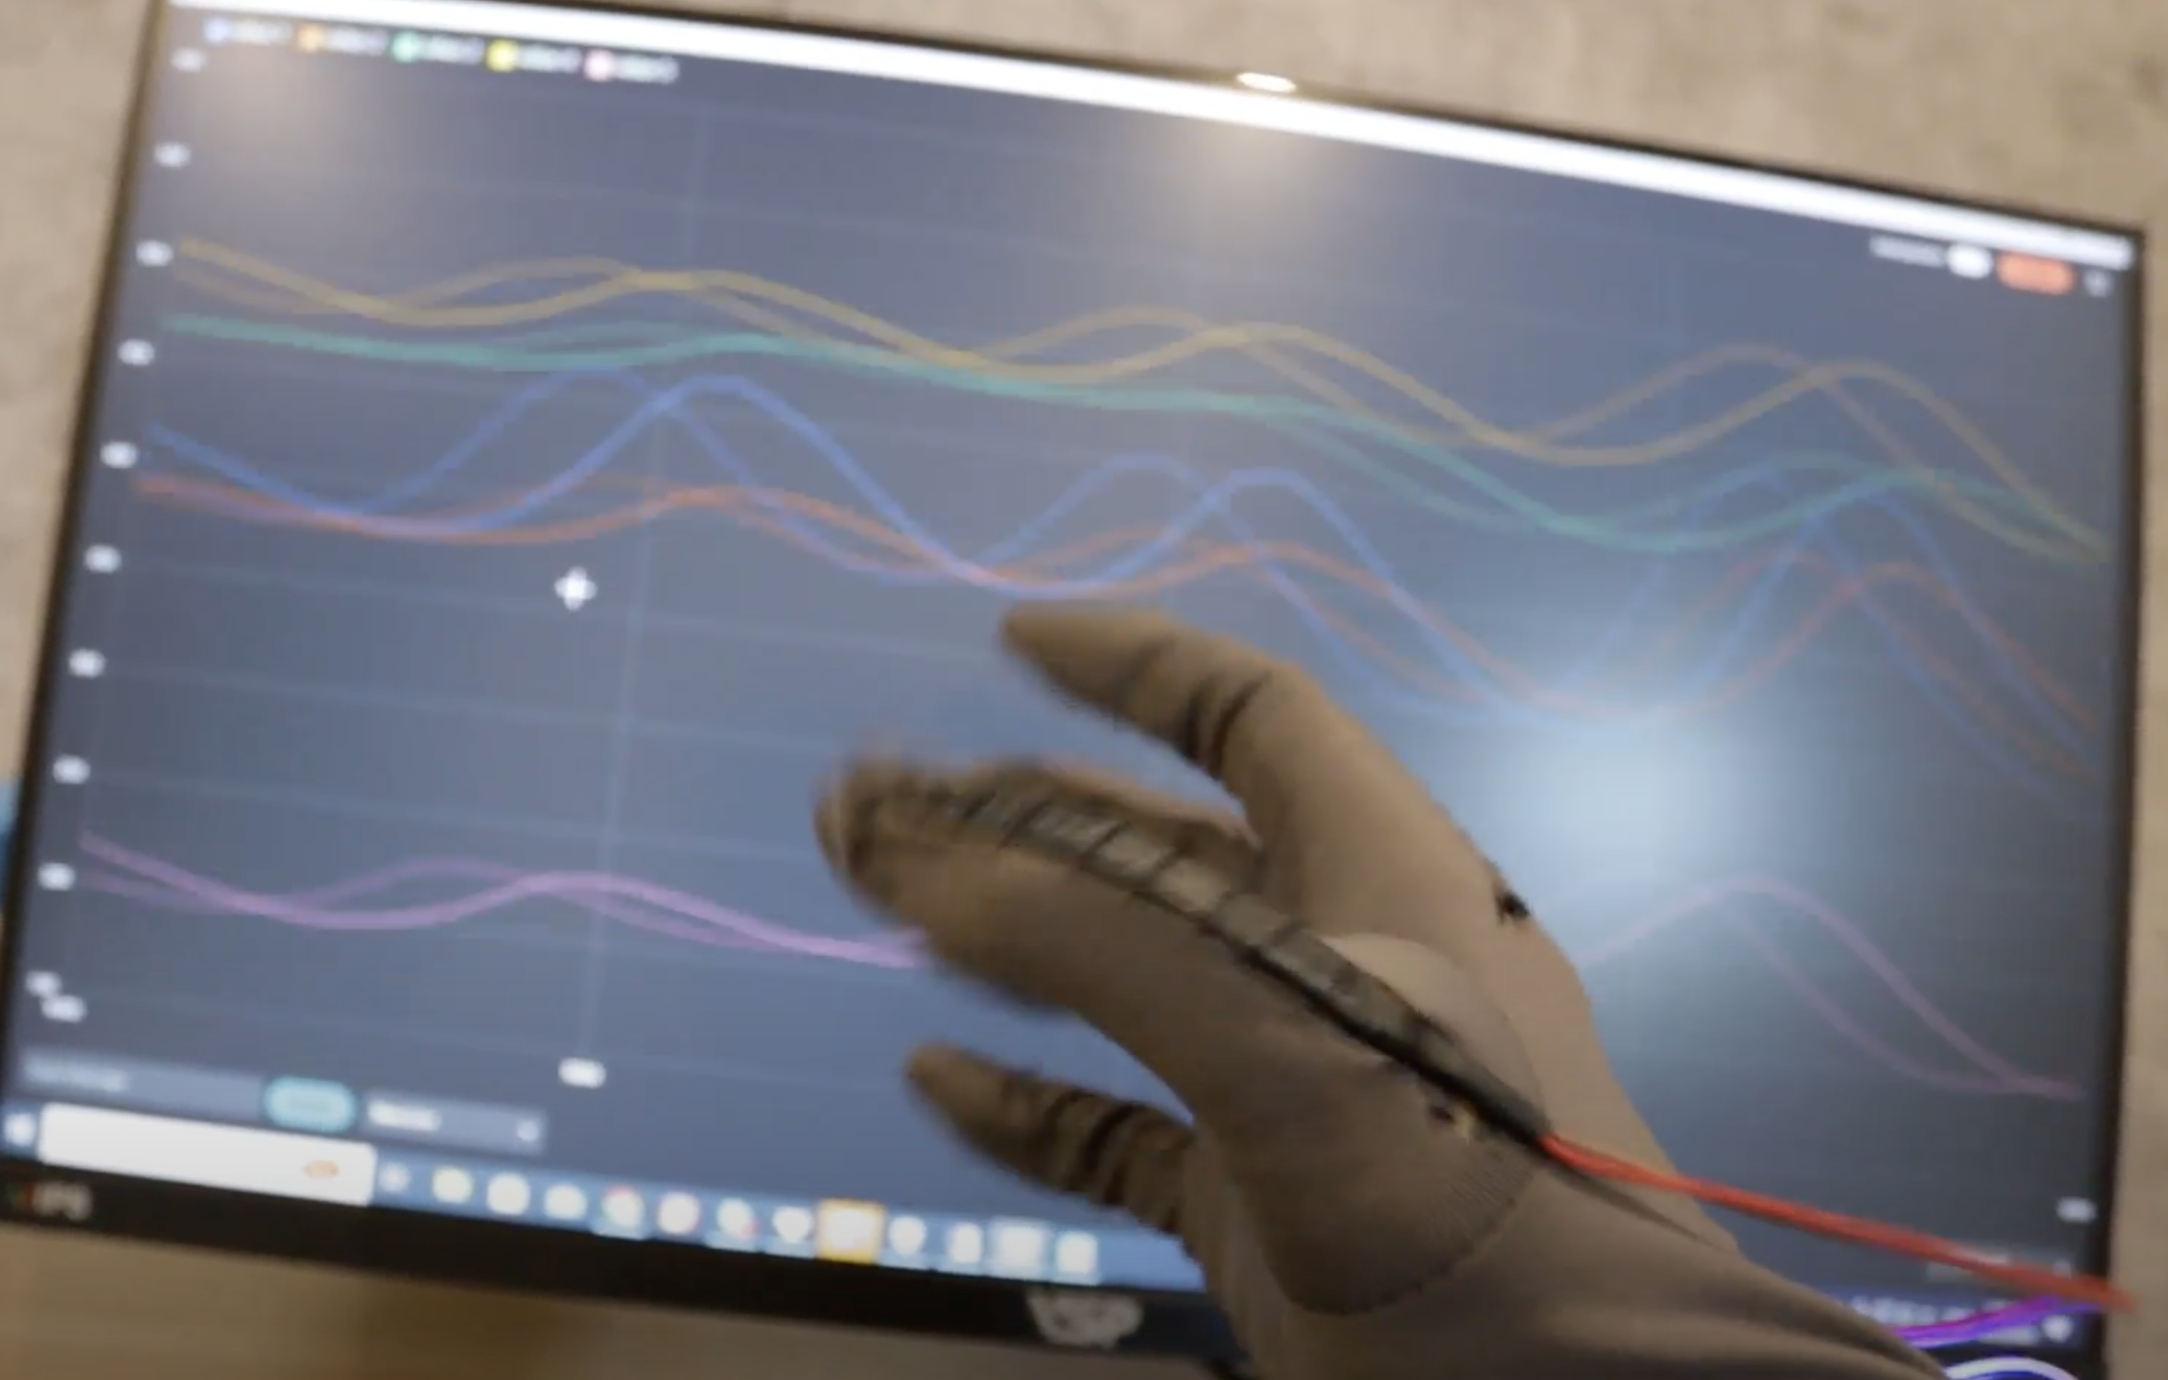
\includegraphics[width=10cm]{Images/SystemImpl/readdt_result_2.png}
\caption{Quá trình lấy dữ liệu}
\end{figure}


% Dữ liệu được thu thập từ module thu thập dữ liệu cử chỉ sau đó được lưu vào file text
% \subsubsection{Dữ liệu được thu thập trên arduino}

% Dữ liêu được gửi từ Arduino có 7 thành phần chính: 

% \begin{lstlisting}
%     gyro.readGyro(&ix,&iy,&iz); 
%     ix = filter_gX.updateEstimate(ix);
%     iy = filter_gY.updateEstimate(iy);
%     iz = filter_gZ.updateEstimate(iz);
%         readFlexSensor(flexSensor);
%     flexSensor[0] = filter_flex0.updateEstimate(flexSensor[0]);
%     flexSensor[1] = filter_flex1.updateEstimate(flexSensor[1]);
%     flexSensor[2] = filter_flex2.updateEstimate(flexSensor[2]);
%     flexSensor[3] = filter_flex3.updateEstimate(flexSensor[3]);
% \end{lstlisting}

% Các dữ liệu được gửi lần lượt là gia tốc trục x, gia tốc trục y, gia tốc trục z, và các tín hiệu analog 1,2,3,4. với flex 1,2 ( ngón trỏ và ngón cái) được nối song song với nhau sau đó nối tiếp đến A0, và các ngón còn lại được nối tuần tự

% Đầu ra của tín hiệu được gửi qua blutetooth có dạng như sau: 
% \begin{lstlisting}
% "%lld\t%lld\t%lld\t%d\t%d\t%d\t%d\n"
% \end{lstlisting}
 
% dữ liệu được gửi với mỗi 10ms một lần



% \subsubsection{Dữ liệu nhận được từ gateway}
% \begin{lstlisting}
% SERIAL_PORT = 'COM5'
% SERIAL_RATE = 38400
% label = 14
% DATA_FILE_NAME = './datatrain1/trainx_'+str(label)+'.txt'  # Specify the output file name
% LABEL_FILE_NAME = './datatrain1/trainy_'+str(label)+'.txt'  # Specify the output file name
% DATA_TEST_FILE_NAME = './datatrain1/testx_'+str(label)+'.txt'  # Specify the output file name
% LABEL_TEST_FILE_NAME = './datatrain1/testy_'+str(label)+'.txt'  # Specify the output file name
% test_counter = 300
% queue_size = 240
% windowSlide = 60
% training_times = 200
% testing_times = 40
% \end{lstlisting}
% \begin{itemize}

% \item\textbf{SERIAL\_PORT} là cổng kết nối với thiết bị
% Sau khi kết nối với bluetooth với arduino, kiểm tra cổng COM đã kết nối bằng cách mở phần mềm arduino

% \begin{figure}[H]
%     \centering
%     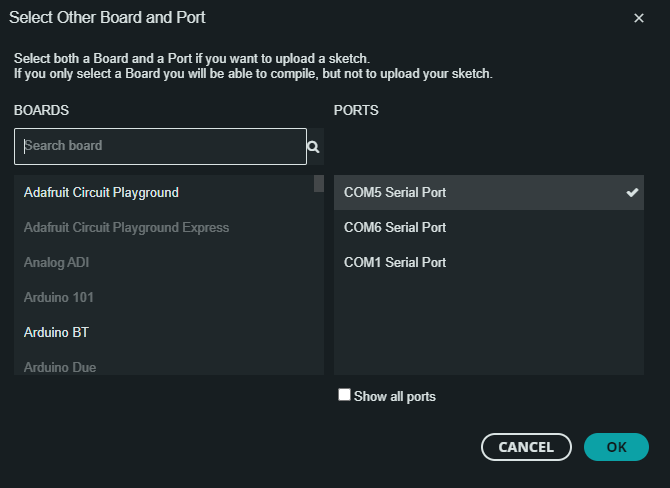
\includegraphics[width=\textwidth,height=\textheight,keepaspectratio]{Images/SystemImpl/checkcomport.png}
%     \caption{kiểm tra các cổng com đang mở}
%     \label{fig:enter-label}
% \end{figure}

% Ví dụ trong bài luận văn này là cổng 5 \\

% \item\textbf{SERIAL\_RATE} ở đây là baudraute khi khởi tạo ở arduino, ở đây module bluetooth HC-05 sử dụng 38400 để đảm bảo thời gian trễ thấp nhất khi một frame dữ liệu được gửi qua\\

% \item\textbf{label} là nhãn của dữ liệu khi được train,nhãn này được định nghĩa ở file config và readme như sau \\

% \begin{longtblr}[
%   caption = {File readme mô tả hành động được thu nhập và gắn nhãn},
% ]{
%   width = \linewidth,
%   colspec = {Q[404]Q[521]},
%   hlines,
%   vlines,
% }
% label 0          & hành động nắm tay  \\
% label 1      & hành động tạm biệt ( hành động chậm)\\
% label 2& hành động tạm biệt ( hành động chậm)\\                              
% label 3 &chỉ vào bản thân (ngón cái đưa lên)\\
% label 4 &không biết ( bàn tay xòe thẳng và xoay quanh trục ngón giữa)\\
% label 5 &trạng thái nghỉ\\
% label 6 &chỉ ra ngoài ( chỉ một ngón trỏ đưa lên) \\
% label 7 &hành động đi bộ ( ngón giữa và ngón trỏ)\\
% label 8 &ngón trỏ chỉ xuống đất và xoay vòng \\
% label 9 &đùa giỡn ( ngón trỏ và ngón giữa co giãn cùng một lúc) \\
% label 10 &chỉ tại đây (ngón cái và ngón giữa chỉ xuống, ngón cái đưa lên )\\
% label 11 &hành động xin chào ( hành động nhanh ) \\
% label 12 &giới thiệu tên \\
% label 13 &thể hiện trạng thái vui vẻ ( bàn tay xòe thẳng và xoay vòng quanh cổ tay ) \\
% label 14 &hành động gặp nhau ( ngón trỏ chỉ lên, các ngón còn lại co )\\
% \end{longtblr}

% \begin{longtblr}[
%   caption = {File config là các đoạn text được chuyển sang giọng nói},
% ]{
%   width = \linewidth,
%   colspec = {Q[404]Q[521]},
%   hlines,
%   vlines,
% }
% Giữ & ~0\\
% Tạm Biệt& ~1\\
% Tốt lắm&~2\\
% Tôi&~3\\
% Không biết&~4\\
% -&~5\\
% Bạn&~6\\
% Đi bộ&~7\\
% Xung quanh&~8\\
% Đùa thôi&~9\\
% Tại đây&~10\\
% Xin chào&~11\\
% Tên là Chánh (điều chỉnh để phát ra tên như mong muốn)&~12\\
% Rất vui&~13\\
% Gặp&~14
% \end{longtblr}

% \item\textbf{DATA\_FILE\_NAME}: nơi lưu trainx\\
% \item\textbf{LABEL\_FILE\_NAME}: nơi lưu trainy\\
% \item\textbf{DATA\_TEST\_FILE\_NAME}: nơi lưu testx\\
% \item\textbf{LABEL\_TEST\_FILE\_NAME}: nơi lưu testy\\
% \item\textbf{test\_counter}: số lần test dữ liệu, được định tính trước khi bắt đầu thu thập \\
% \item\textbf{queue\_size}: một frame dữ liệu để gắn nhãn cho frame đó\\
% \item\textbf{windowSlide}: cửa số trượt, một lượng dữ liệu một để thêm vào một frame, trùng lặp với frame trước đó được tính bằng $queue\_size - windowSlide$
% \item\textbf{training\_times}: số frame dữ liệu được ghi vào file train
% \item\textbf{testing\_times}: số frame dữ liệu được ghi vào file test
% \end{itemize}

% Tiến hành thu thập dữ liệu với các động tác tay được định nghĩa như ở file readme


% Các file data được lưu có kích thước cho một hành động như sau 
% \begin{itemize}
%     \item Một hàng có 240*7 cột dữ liệu
%     \item Có tổng cộng 200 hàng dữ liệu cho file train và 20 cho trainy 
% \end{itemize}
\newpage
\subsection{Định dạng dữ liệu trước khi đưa vào học máy}

Phần này tập trung vào việc chuẩn bị và chuyển đổi dữ liệu từ tệp lưu trữ thành định dạng phù hợp để sử dụng trong mô hình học máy. Quy trình được thực hiện như sau:

\subsubsection{Đọc và tổ chức dữ liệu}

\begin{itemize}
    \item \textbf{Dữ liệu đầu vào:} Dữ liệu được đọc từ các tệp:
    \begin{itemize}
        \item \texttt{trainx} và \texttt{testx}: Chứa dữ liệu đầu vào từ các cảm biến.
        \item \texttt{trainy} và \texttt{testy}: Chứa nhãn tương ứng cho các mẫu dữ liệu đầu vào.
    \end{itemize}

    \item \textbf{Quy trình xử lý:}
    \begin{itemize}
        \item Mỗi dòng dữ liệu trong tệp đầu vào chứa 1680 giá trị, được chia thành 7 chuỗi (tương ứng với 7 giá trị cảm biến) và 240 bước thời gian.
        \item Dữ liệu được tách ra và chuyển đổi thành ma trận 3 chiều với kích thước $(\text{số mẫu}, 240, 7)$.
    \end{itemize}
\end{itemize}

\subsubsection{Định dạng dữ liệu đầu vào}

\begin{itemize}
    \item \textbf{Kết hợp giá trị cảm biến:}
    \begin{itemize}
        \item Sử dụng hàm \texttt{dstack} để kết hợp dữ liệu từ 7 cảm biến thành ma trận.
        \item Mỗi mẫu có định dạng:
        \[
        (240, 7)
        \]
        Trong đó:
        \begin{itemize}
            \item $240$: Số bước thời gian (sequence length).
            \item $7$: Số lượng đặc trưng (gia tốc các trục X, Y, Z và tín hiệu từ các cảm biến Flex).
        \end{itemize}
    \end{itemize}

    \item \textbf{Định dạng đầu ra:}
    \begin{itemize}
        \item Chuyển nhãn (\texttt{trainy} và \texttt{testy}) sang định dạng one-hot encoding bằng hàm \texttt{to\_categorical}.
        \item Kích thước nhãn sau khi chuyển đổi:
        \[
        (\text{số mẫu}, \text{số lớp})
        \]
    \end{itemize}
\end{itemize}

\subsubsection{Chuẩn hóa dữ liệu}

\begin{itemize}
    \item Sử dụng các công cụ từ thư viện \texttt{sklearn} để chuẩn hóa dữ liệu:
    \begin{itemize}
        \item \texttt{StandardScaler}: Chuẩn hóa các giá trị về trung bình 0 và phương sai 1.
        \item \texttt{MinMaxScaler}: Đưa dữ liệu về khoảng [0, 1].
    \end{itemize}
\end{itemize}

\subsubsection{Chuẩn bị dữ liệu cho mô hình LSTM}

Dữ liệu được tổ chức thành hai tập chính:
\begin{itemize}
    \item \textbf{Tập huấn luyện} (\texttt{trainX} và \texttt{trainy}):
    \begin{itemize}
        \item Đầu vào: Ma trận $(\text{số mẫu huấn luyện}, 240, 7)$.
        \item Đầu ra: Ma trận $(\text{số mẫu huấn luyện}, \text{số lớp})$ (one-hot encoding).
    \end{itemize}

    \item \textbf{Tập kiểm tra} (\texttt{testX} và \texttt{testy}):
    \begin{itemize}
        \item Đầu vào: Ma trận $(\text{số mẫu kiểm tra}, 240, 7)$.
        \item Đầu ra: Ma trận $(\text{số mẫu kiểm tra}, \text{số lớp})$.
    \end{itemize}
\end{itemize}

\subsubsection{Định nghĩa đầu vào và đầu ra của mô hình}

\begin{itemize}
    \item \textbf{Đầu vào:}
    \begin{itemize}
        \item Chuỗi thời gian có chiều $(240, 7)$, đại diện cho các tín hiệu liên tục từ cảm biến.
    \end{itemize}

    \item \textbf{Đầu ra:}
    \begin{itemize}
        \item Xác suất dự đoán của từng lớp, biểu diễn bằng một vector có chiều $(\text{số lớp})$.
    \end{itemize}
\end{itemize}

\subsubsection{Tóm tắt}

Quy trình định dạng dữ liệu bao gồm các bước xử lý từ tệp dữ liệu thô đến định dạng đầu vào/đầu ra phù hợp với mô hình LSTM. Điều này đảm bảo dữ liệu có cấu trúc rõ ràng và đáp ứng yêu cầu của mô hình học máy, góp phần nâng cao hiệu quả và độ chính xác trong quá trình huấn luyện.

% \subsection{Định dạng data trước khi đưa vào học máy}
% \begin{lstlisting}
% line = next(testx).strip().split()
%                 if len(line) >= 1680:
%                     for i in range(240):
%                         x1.append(int(line[i]))
%                         x2.append(int(line[i + 240]))
%                         x3.append(int(line[i + 480]))
%                         x4.append(int(line[i + 720]))
%                         x5.append(int(line[i + 960]))
%                         x6.append(int(line[i + 1200]))
%                         x7.append(int(line[i + 1440]))
%                 else:
%                     print("Error test data.")
%                 x1 = array(x1)
%                 x2 = array(x2)
%                 x3 = array(x3)
%                 x4 = array(x4)
%                 x5 = array(x5)
%                 x6 = array(x6)
%                 x7 = array(x7)
%                 line_dataset = dstack([x1, x2, x3, x4, x5, x6, x7]) 
%                 line_dataset = line_dataset.reshape(1,240,7)
%                 testx_data.append(line_dataset)
% \end{lstlisting}

% Có hai loại tín hiệu chính trong dữ liệu gốc: gia tốc và flexsensor
% Gia tốc có 3 trục dữ liệu, flexsensor có 4 trục dữ liệu
% mỗi loạt dữ liệu được ghi với thời gian là 2.4 giây
% tương đương với 240 bước thời gian. Các cửa sổ dữ liệu này tương ứng với các cửa sổ đặc trưng đã được tạo ra trước đó. Điều này có nghĩa là một hàng dữ liệu có (240 * 7), tức là 1680 phần tử.

% Dữ liệu sau khi được tải từ file text, sau đó được phân chia thành từng frame dữ liệu:\\
% Mỗi frame dữ liệu có các tính chất như sau:
% \begin{itemize}
% \item Mỗi cột dữ liệu được ghi 240 lần 
% \item Có tổng cộng 7 cột dữ liệu tương ứng với 7 feature của một frame

% \end{itemize}
% Có thể thấy hàm reshape sẽ đảm nhận việc đó
\newpage
\subsection{Xây dựng mô hình học máy}

Mô hình học máy được xây dựng sử dụng kiến trúc LSTM (Long Short-Term Memory) nhằm xử lý dữ liệu chuỗi thời gian từ các cảm biến và nhận diện chính xác các cử chỉ ngôn ngữ ký hiệu.

\subsubsection{Cấu trúc của mô hình}

Mô hình được xây dựng với các thành phần chính sau:
\begin{itemize}
    \item \textbf{LSTM Layer:}
    \begin{itemize}
        \item Lớp LSTM đầu tiên với 128 đơn vị (units), nhận đầu vào có kích thước $(240, 7)$ tương ứng với 240 bước thời gian và 7 đặc trưng từ cảm biến.
        \item Lớp này có tổng cộng \textbf{69,632 tham số} được tối ưu trong quá trình huấn luyện.
    \end{itemize}

    \item \textbf{Dropout Layer:}
    \begin{itemize}
        \item Lớp Dropout với tỷ lệ rơi rụng là 50\% giúp giảm thiểu hiện tượng overfitting trong quá trình huấn luyện.
        \item Lớp này không bổ sung thêm tham số nào.
    \end{itemize}

    \item \textbf{Flatten Layer:}
    \begin{itemize}
        \item Lớp Flatten chuyển đổi đầu ra từ LSTM thành vector phẳng, kích thước $(128)$.
        \item Lớp này không có tham số học.
    \end{itemize}

    \item \textbf{Dense Layer:}
    \begin{itemize}
        \item Lớp Dense ẩn với 64 đơn vị (units) và hàm kích hoạt ReLU.
        \item Lớp này bổ sung \textbf{8,256 tham số}.
    \end{itemize}

    \item \textbf{Output Dense Layer:}
    \begin{itemize}
        \item Lớp đầu ra với 5 đơn vị tương ứng với số lớp trong bài toán phân loại.
        \item Sử dụng hàm kích hoạt softmax để chuyển đổi đầu ra thành xác suất.
        \item Lớp này bổ sung \textbf{325 tham số}.
    \end{itemize}
\end{itemize}

\subsubsection{Tổng số tham số}

\begin{itemize}
    \item Tổng số tham số học được trong mô hình: \textbf{78,213 tham số}.
    \item Mô hình không chứa tham số không thể học (non-trainable).
\end{itemize}

\subsubsection{Quy trình xây dựng mô hình}

\begin{itemize}
    \item \textbf{Khởi tạo mô hình:}
    \begin{itemize}
        \item Mô hình được khởi tạo sử dụng API tuần tự (\texttt{Sequential}) của Keras.
    \end{itemize}

    \item \textbf{Thêm các lớp vào mô hình:}
    \begin{itemize}
        \item Lớp LSTM đầu tiên nhận đầu vào có kích thước $(240, 7)$ và trả về đầu ra có kích thước $(128)$.
        \item Thêm lớp Dropout với tỷ lệ 0.5.
        \item Thêm lớp Flatten để làm phẳng đầu ra của LSTM.
        \item Thêm lớp Dense ẩn với 64 đơn vị và hàm kích hoạt ReLU.
        \item Thêm lớp Dense đầu ra với 5 đơn vị và hàm kích hoạt softmax.
    \end{itemize}

    \item \textbf{Biên dịch mô hình:}
    \begin{itemize}
        \item Sử dụng hàm mất mát \texttt{categorical\_crossentropy} để tối ưu hóa bài toán phân loại.
        \item Trình tối ưu \texttt{adam} được lựa chọn để đảm bảo quá trình học nhanh chóng và hiệu quả.
        \item Đo lường hiệu suất bằng độ chính xác (\texttt{accuracy}).
    \end{itemize}

    \item \textbf{Huấn luyện mô hình:}
    \begin{itemize}
        \item Số \texttt{epoch}: 300.
        \item Kích thước \texttt{batch}: 4,500 mẫu mỗi lần cập nhật trọng số.
        \item Bộ dữ liệu đầu vào và nhãn được đưa vào quá trình huấn luyện thông qua hàm \texttt{model.fit()}.
    \end{itemize}
\end{itemize}

\subsubsection{Tóm tắt mô hình}

\begin{table}[h]
\centering
\caption{Bảng tóm tắt mô hình}
\begin{tabular}{|l|l|r|}
\hline
\textbf{Layer (type)} & \textbf{Output Shape} & \textbf{Param \#} \\ \hline
LSTM                 & (None, 128)            & 69,632           \\ \hline
Dropout              & (None, 128)            & 0                \\ \hline
Flatten              & (None, 128)            & 0                \\ \hline
Dense                & (None, 64)             & 8,256            \\ \hline
Dense                & (None, 5)              & 325              \\ \hline      
\textbf{Total}       &                        & \textbf{78,213}  \\ \hline
\end{tabular}

\end{table}

\begin{itemize}
    \item Tổng số tham số: 78,213
    \item Kích thước bộ tham số: ~305.52 KB  
\end{itemize}


\subsubsection{Tóm tắt}

Mô hình LSTM được xây dựng và tối ưu hóa để xử lý dữ liệu chuỗi thời gian từ cảm biến. Với cấu trúc đơn giản nhưng hiệu quả, mô hình có khả năng phân loại chính xác các cử chỉ ngôn ngữ ký hiệu, đồng thời đảm bảo tính tổng quát khi áp dụng trên tập dữ liệu kiểm tra.











